\documentclass{article}
\usepackage[utf8]{inputenc}
\usepackage[table]{xcolor} % For cell coloring
\usepackage{geometry} % For page margins
\usepackage{graphicx} % For including images
\usepackage{float} % For image placement
\usepackage{tabularx} % For table stretching
\usepackage{multirow}
\usepackage{colortbl}
\usepackage{xspace}
\usepackage{hyperref}
\usepackage{parskip}
\usepackage{amsmath}

\usepackage{listings}


\usepackage{titlesec}
\titleformat{\subparagraph}
    {\normalfont\normalsize\bfseries}{\thesubparagraph}{1em}{}
\titlespacing*{\subparagraph}{\parindent}{3.25ex plus 1ex minus .2ex}{.75ex plus .1ex}


\input{/home/oddish3/Documents/uni/mast-2/preamble.tex}
\input{/home/oddish3/Documents/uni/mast-2/notation.tex}

% Moment Test and Descriptive Statistics
\newcommand{\amu}{0.10\xspace}
\newcommand{\asigma}{1.83\xspace}
\newcommand{\askew}{-0.32\xspace}
\newcommand{\akurt}{4.26\xspace}
\newcommand{\amut}{0.83\xspace}
\newcommand{\askewt}{-2.08\xspace}
\newcommand{\akurtt}{4.06\xspace}
\newcommand{\ajbt}{20.85\xspace}
\newcommand{\amup}{0.40\xspace}
\newcommand{\askewp}{0.04\xspace}
\newcommand{\akurtp}{0.00\xspace}
\newcommand{\ajbp}{0.00\xspace}

% Ljung-Box Test Results
\newcommand{\aistat}{27.06\xspace}
\newcommand{\aip}{0.17\xspace}
\newcommand{\aiistat}{25.61\xspace}
\newcommand{\aiip}{0.22\xspace}

% GARCH(1,1) with zt ~ N(0,1)
\newcommand{\bw}{2.53\xspace}
\newcommand{\ba}{0.13\xspace}
\newcommand{\bb}{0.15\xspace}
\newcommand{\bpi}{0.54\xspace}
\newcommand{\bpii}{0.03\xspace}
\newcommand{\bpiii}{0.90\xspace}

% GARCH(1,1) with zt ~ tv
\newcommand{\bwi}{0.24\xspace}
\newcommand{\bai}{0.07\xspace}
\newcommand{\bbi}{0.87\xspace}
\newcommand{\bvi}{4.62\xspace}
\newcommand{\bpti}{0.58\xspace}
\newcommand{\bptii}{0.22\xspace}
\newcommand{\bptiii}{0.00\xspace}
\newcommand{\bptiv}{0.00\xspace}

% GJR-GARCH(1,1) with zt ~ N(0,1)
\newcommand{\bwii}{3.06\xspace}
\newcommand{\baii}{0.00\xspace}
\newcommand{\bbii}{0.00\xspace}
\newcommand{\bgii}{0.29\xspace}
\newcommand{\bpgi}{0.02\xspace}
\newcommand{\bpgii}{1.00\xspace}
\newcommand{\bpgiii}{1.00\xspace}
\newcommand{\bpgiv}{0.19\xspace}

% GJR-GARCH(1,1) with zt ~ tv
\newcommand{\bwiii}{0.22\xspace}
\newcommand{\baiii}{0.02\xspace}
\newcommand{\bbiii}{0.89\xspace}
\newcommand{\bgiii}{0.07\xspace}
\newcommand{\bviii}{4.57\xspace}
\newcommand{\bpgtp}{0.26\xspace}
\newcommand{\bpgtpi}{0.57\xspace}
\newcommand{\bpgtpii}{0.00\xspace}
\newcommand{\bpgtpiii}{0.13\xspace}
\newcommand{\bpgtpiv}{0.00\xspace}

% residuals and squared lbq
\newcommand{\zone}{12.80\xspace}
\newcommand{\pone}{0.92\xspace}
\newcommand{\zfive}{16.87\xspace}
\newcommand{\pfive}{0.72\xspace}
\newcommand{\ztwo}{12.39\xspace}
\newcommand{\ptwo}{0.93\xspace}
\newcommand{\zsix}{16.21\xspace}
\newcommand{\psix}{0.76\xspace}
\newcommand{\zthree}{13.09\xspace}
\newcommand{\pthree}{0.91\xspace}
\newcommand{\zseven}{18.23\xspace}
\newcommand{\pseven}{0.63\xspace}
\newcommand{\zfour}{13.04\xspace}
\newcommand{\pfour}{0.91\xspace}
\newcommand{\zeight}{17.85\xspace}
\newcommand{\peight}{0.66\xspace}

% root mean square forecast error and dm test
\newcommand{\rmsfei}{1.16\xspace}
\newcommand{\rmsfeii}{1.10\xspace}
\newcommand{\rmsfeiii}{1.23\xspace}
\newcommand{\rmsfeiv}{1.11\xspace}
\newcommand{\dm}{0.84\xspace}
\newcommand{\dmpii}{0.72\xspace}
\newcommand{\dmi}{-0.94\xspace}
\newcommand{\dmpiv}{0.26\xspace}
\newcommand{\dmii}{0.75\xspace}
\newcommand{\dmpv}{0.70\xspace}


% Define colours
\definecolor{headercolor}{RGB}{169,169,169} % Grey color, adjust the RGB values as per your document
\definecolor{rowcolor}{RGB}{255,255,255} % White color, adjust if your document has a different row color

% Set page margins
\geometry{left=25mm,right=25mm,top=25mm,bottom=25mm}

% Custom column type for tabularx
\newcolumntype{Y}{>{\centering\arraybackslash}X}

\title{ECON60332 Coursework Template}
\author{Group 11} % INSERT GROUP NUMBER HERE
\date{}

\begin{document}

\maketitle

\noindent\begin{tabularx}{\linewidth}{|Y|Y|}
    \hline
    \rowcolor{headercolor} Participant’s Student ID & Indicate if the student did not participate \\
    \hline
    \multicolumn{1}{|c|}{10710007}\\
    \hline

\end{tabularx}

\section*{Theoretical exercise}

\subsection*{Question a}

When comparing the ARCH(2) model : $\sigma^2_{t} = \omega + \alpha_1 \epsilon_{t-1}^2 + \alpha_2 \epsilon^2_{t-2})$ to a GARCH(1,1)) : $\sigma^2_{t} = \omega + \alpha_1 \epsilon_{t-1}^2 + \beta_2 \sigma^2_{t-1})$

The following similarities emerge :
\begin{itemize}
	\item Both models capture the cluster effect where periods of high (low) volatility are followed by periods of high (low) volatility (probabilistically) 
		\item Both model capture overkurtosis, accounting for a heavier tail distribution than the standard norm
		\item If $z_{t}$ is not symmetric, then $\cov(\epsilon_t, \sigma^2_{t+1} | \ensuremath{\mathcal{F}}_{t-1})$ would not be zero, and both model are able to capture leverage (asymmetric) effects 
\end{itemize}

Though with key differences that
\begin{itemize}
	\item An arch model implies an AR model for the squared residuals whilst a GARCH model implies an ARMA model in both squared residuals and variance
	\item Fir the GARCH model $b_1$ can be unidentified if $a_1=0$
\end{itemize}

\subsection*{Question b}

Assuming $\alpha_1 + \alpha_2 < 1$ for stationarity

Where \( \mathcal{F}_{t-1} \) is the past history of the process, then the conditional expectation of \( \epsilon_t \) is given by:
\begin{equation}
	E(\epsilon_t | \mathcal{F}_{t-1}) = E(\sqrt{\sigma^2_t } z_{t}| \mathcal{F}_{t-1}) = \sigma_t E(z_t | \mathcal{F}_{t-1}) = \sigma_t \cdot 0 = 0
\end{equation}
Using LIE, we can obtain the unconditional mean :
\begin{equation}
E(\epsilon_t) = E(E(\epsilon_t | \mathcal{F}_{t-1})) = E(0) = 0
\end{equation}

To derive the second moment, we can express \( \epsilon_t^2 \) as an AR(22)-process:

\begin{align*}
\sigma^2_t + \epsilon^2_{t} = \omega + \alpha_1 \epsilon_{t-1}^2 + \alpha_2 \epsilon_{t-2}^2 + \epsilon^2_{t} \\
\epsilon_t^2 = \omega + \alpha_1 \epsilon_{t-1}^2 + \alpha_2 \epsilon_{t-2}^2 + \nu_t
\end{align*}
with \( \nu_t = \epsilon_t^2 - \sigma_t^2 \) being a WN process.

It holds that:
\begin{equation}
E(\epsilon^2_t | \mathcal{F}_{t-1}) = E(\sigma^2_t  z^2_{t}| \mathcal{F}_{t-1}) = \sigma^2_t E(z^2_t | \mathcal{F}_{t-1}) = \sigma^2_t \cdot 1 = \sigma^2_t
\end{equation}

Such that:
\begin{equation}
E(\nu_t | \mathcal{F}_{t-1}) = E(\epsilon_t^2 | \mathcal{F}_{t-1}) - \sigma_t^2 = \sigma_t^2 - \sigma_t^2 = 0
\end{equation}

Therefore:
\begin{equation}
E(\nu_t) = E(E(\nu_t | \mathcal{F}_{t-1})) = E(0) = 0
\end{equation}

Which allows us to write:
\begin{align*}
E(\epsilon_t^2) = \omega + \alpha_1 E \left[   \epsilon_{t-1}^2 \right] + \alpha_2  E \left[ \epsilon_{t-2}^2 \right] + E \left[ \nu_t \right] \\
&= \omega + \alpha_1 E \left[ \epsilon_{t-1}^2 \right] + \alpha_2  E \left[ \epsilon_{t-2}^2 \right]
\end{align*}

Using stationarity, \( E(\epsilon_{t-1}^2) = E(\epsilon_t^2) \) and hence we conclude that:

\begin{align*}
\mathrm{Var}(\epsilon_t) = E(\epsilon_t^2) - (E(\epsilon_t))^2 = E(\epsilon_t^2) =  \omega + \alpha_1 \mathrm{Var}(\epsilon_{t-1}) - \alpha_2 \mathrm{Var}(\epsilon_{t-2}) = \frac{\omega}{1- \alpha_1 - \alpha_2} = \frac{\omega}{1 - \sum_{i=1}^{2} \alpha_{i} } 
\end{align*}

\subsection*{Question c}

Using the covariance definition $\text{Cov}(X, Y) = E[XY] - E[X]E[Y]$ and given the conditional variance $\sigma^2_{t+1} = \omega + \alpha_1 \epsilon_{t}^2 + \alpha_2 \epsilon^2_{t-1}$, we derive the covariance as follows:
\begin{align*}
\text{Cov}(\sigma^2_{t+1}, \epsilon_t | \mathcal{F}_{t-1}) &= E[\sigma^2_{t+1} \epsilon_t | \mathcal{F}_{t-1}] - E[\sigma^2_{t+1} | \mathcal{F}_{t-1}]E[\epsilon_t | \mathcal{F}_{t-1}] \\
&= E[\sigma^2_{t+1} \epsilon_t | \mathcal{F}_{t-1}] - 0 \\
&= E \left[ \left( \omega + \alpha_1 \epsilon_{t}^2 + \alpha_2 \epsilon^2_{t-1} \right) \epsilon_t | \mathcal{F}_{t-1} \right] \\
&= \omega E[\epsilon_t | \mathcal{F}_{t-1}] + \alpha_1 E[\epsilon_t^3 | \mathcal{F}_{t-1}] + \alpha_2 E[\epsilon^2_{t-1} \epsilon_t | \mathcal{F}_{t-1}] \quad \text{(since $\omega$ and $\epsilon^2_{t-1}$ don't depend on $\epsilon_t$}) \\
&= 0 + \alpha_1 E[\epsilon_t^3 | \mathcal{F}_{t-1}] + 0 \quad \text{(since $\epsilon_t$ is conditionally zero-mean and independent of $\epsilon_{t-1}$)}.
\end{align*}

Now, if we consider $\epsilon_t = \sigma_t z_t$ :
\begin{align*}
\text{Cov}(\sigma^2_{t+1}, \epsilon_t | \mathcal{F}_{t-1}) =
\alpha_1 E[\epsilon_t^3 | \mathcal{F}_{t-1}] &= \alpha_1 E[(\sigma_t z_t)^3 | \mathcal{F}_{t-1}] \\
&= \alpha_1 \sigma_t^3 E[z_t^3 | \mathcal{F}_{t-1}] \\
&= \alpha_1 \left( \omega + \alpha_1 \epsilon_{t}^2 + \alpha_2 \epsilon^2_{t-1} \right)^\frac{3}{2} E[z_t^3].
\end{align*}
Only with  non-zero third moment on $z_t$, is the model able to capture the leverage (asymmetric) effect.   
Since $z_t ~ \mathcal{N}(0,\,1)$ , the third moment is 0 and $\text{Cov}(\sigma^2_{t+1}, \epsilon_t | \mathcal{F}_{t-1}) = 0$ so the model cannot capture the leverage effect, which is the tendency for negative shocks to have a different impact on volatility than positive shocks.

\subsection*{Question d}

With our ARCH(2) model, the 1 step ahead forecast is : $\sigma^2_{t+1 | t}  = \omega + \alpha_1  \epsilon^2_{t}  + \alpha_2  \epsilon^2_{t-1}$

Analogously the 2 step ahead forecast, where we take expectation of $\epsilon_t^2$, and use the unit variance of $z_{t}$ to simplify 
\begin{align*}
\sigma^2_{t+2 | t}  = E_t \left[  \omega + \alpha_1  \epsilon^2_{t+1}  + \alpha_2  \epsilon^2_{t}  \right] =   \omega + \alpha_1  \sigma^2_{t+1|t}  + \alpha_2  \sigma^2_{t}  
\end{align*}

Similarly for the 3-step ahead forecast, following the same logic

 \begin{align*}
 	\sigma^2_{t+3 | t} = E_t \left[  \omega + \alpha_1  \epsilon^2_{t+2}  + \alpha_2  \epsilon^2_{t+1}  \right] =   \omega + \alpha_1  \sigma^2_{t+2|t}  + \alpha_2  \sigma^2_{t+1} \equiv E \left[ \sigma^2_{t+3} | F_{t} \right] 
 \end{align*}

\subsection*{Question e}

The news impact curve illustrates how a shock to \( \epsilon_{t-1} \) affects \( \sigma_t^2 \).

We derive the unconditional long-term variance \( \bar{\sigma}^2 \) assuming that \( E(\epsilon_t^2) \) at any point is equal to \( \bar{\sigma}^2 \). From the stationarity condition:
\begin{equation}
E(\epsilon_t^2) = \omega + \alpha_1 E(\epsilon_{t-1}^2) + \alpha_2 E(\epsilon_{t-2}^2).
\end{equation}
Given \( E(\epsilon_{t-1}^2) = E(\epsilon_{t-2}^2) = \bar{\sigma}^2 \), the equation simplifies to:
\begin{equation}
\bar{\sigma}^2 = \frac{\omega}{1 - \alpha_1 - \alpha_2}.
\end{equation}

The news impact curve for the ARCH(2) model is then set up as:
\begin{equation}
\sigma_t^2 = \omega + \alpha_1 \epsilon_{t-1}^2 + \alpha_2 \bar{\sigma}^2.
\end{equation}
With the most recent shock \( \epsilon_{t-1} \) highlighted, we rewrite it as:
\begin{equation}
\sigma_t^2 = A + \alpha_1 \epsilon_{t-1}^2,
\end{equation}
where \( A = \omega + \alpha_2 \bar{\sigma}^2 \)

Thus with an asymmetric distribution, we can derive the NIC as :

\begin{equation}
\text{NIC}(\epsilon_{t-1} | \sigma_{t-1}^2 = \sigma_Y^2) = \omega + \alpha_1 \epsilon_{t-1}^2 + \alpha_2 \sigma_Y^2.
\end{equation}

\section*{Practical exercise}
\subsection*{Question a}

\begin{table}[H]
\centering
\begin{tabular}{|l|c|c|c|c|}
\hline
\rowcolor{headercolor}
 & Sample moments & & Test statistic & P-value \\
\hline
Mean & \amu &   Mean & \amut & \amup \\
\hline
Standard deviation & \asigma &  Skewness & \askewt & \askewp \\
\hline
Skewness &  \askew & Kurtosis & \akurtt & \akurtp \\
\hline
Kurtosis & \akurt & JB & \ajbt & \ajbp \\
\hline
\end{tabular}
\end{table}

\subsection*{LBQ test results:}
\noindent\begin{tabularx}{\linewidth}{|Y|Y|Y|}
    \hline
    \rowcolor{headercolor} & Returns & Squared returns \\
    \hline
    Test statistic & \aistat & \aiistat \\
    \hline
    P-value & \aip & \aiip \\
    \hline
\end{tabularx}

\subsubsection*{Plot of Daily Log Returns}

\begin{figure}[H]
    \centering
    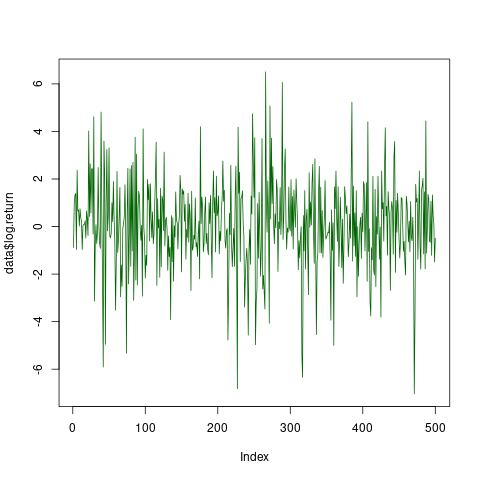
\includegraphics[width=0.35\textwidth]{../../docs/figures/log_return_plot.png}
    \caption{Log Return Plot}
    \label{fig:logreturn}
\end{figure}

\subsubsection*{SACF and SPACF}

\begin{figure}[H]
    \centering
    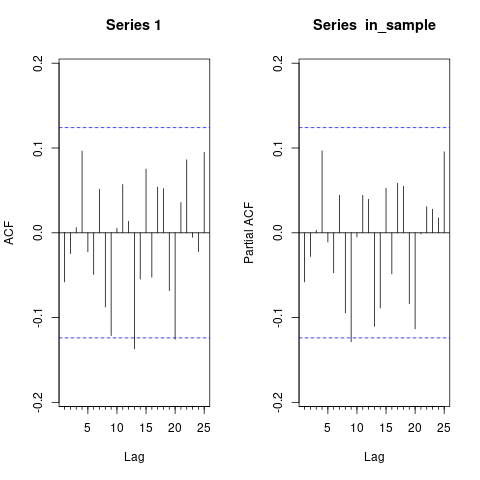
\includegraphics[width=0.35\textwidth]{../../docs/figures/PACF.png}
    \caption{Sample Autocorrelation and Partial Autocorrelation Function Plot}
    \label{fig:pacf}
\end{figure}

\subsection*{Interpretation}
Looking at the Descriptive Statistics, a skewness of \askew suggests that the distribution of returns negatively skewed, meaning there are more extreme negative returns than positive returns. 
Whilst a kurtosis of \akurt is slightly higher than a normal distribution (3), suggesting the distribution of returns has heavier tails and more extreme values.

Looking at the Test Statistics, testing mean returns are zero ($H_0 : \mu =0$ against $H_1 : \mu \neq = 0$) with a one-sided test.
Obtaining \amut with a p-value of \amup, we fail to reject $H_0$ at all conventional significance levels, since we do not have enough evidence to conclude the mean return is significantly different from zero. 

Testing the skewness of the return series is zero ($ H_1: \gamma = 0$ against $H_1 : \gamma \neq = 0$)
We obtain \askewt with a p-value of \askewp, since the p-value is less than 0.05, we reject the null hypothesis in favour of the alternative hypothesis. 
Thus, the distribution of returns is significantly skewed, and hence non-symmetric. 
Testing for leptokurtic property in the returns ($H_0 : \kappa = 3$ against $H_1 : \kappa \neq 3 $)
We obtain \akurt and p value of $\akurtp$, thus we reject $H_0$, in favour of the alternative hypothesis that the returns have significantly different kurtosis from 3, confirming the presence of heavy tails in the distribution. 

Using the Jargue-Bera test for normality ($H_0 : \gamma = 0 \& \kappa = 3$ against $H_0 : \gamma \neq 0 \& \kappa \neq 3$) 

Obtaining \ajbt with a p-value of \ajbp, we reject $H_0$ in favour of $H_1$, that the distribution of returns differs significantly from normality, evidence by its skewness and kurtosis values. 

Testing the autocorrelation of the financial time series returns ($H_0: \rho_1 = \rho_2 = \ldots = \rho_{21} = 0$ against $H_1: \rho_i \neq 0$ for some $i \in \{1, 2, \ldots, 21 \}$)

Obtaining a p-value of 0.17, we do not reject the null hypothesis at all conventional significance levels, thus, there is no significant evidence of autocorrelation in the returns of the series.
We proceed analogously for the squared returns, arriving at the same conclusion, indicating no significant evidence of autocorrelation in the volatility (squared returns) of the series. 

For the plots, there is no consistent pattern of significant lags in both plots, however a significant negative correlation at lag 13 alongside lags approaching significance at 9 and 20 suggests some evidence for a seasonal pattern, however the presence of significant lags informs us the time series is not white noise and exhibits some autocorrelation. 

The Daily Log-returns plot does not display a clear trend or seasonal pattern, although the volatility appears to be clustered in certain periods, indicative of heteroskedacity.

\subsection*{Question b}

\begin{table}[H]
\centering
\begin{tabular}{|c|c|c|c|c|c|}
\hline
\rowcolor{gray!50}
\multicolumn{3}{|c|}{GARCH} & \multicolumn{3}{|c|}{GJR-GARCH} \\ 
\hline
Parameter & Estimate & P-value & Parameter & Estimate & P-value \\ 
\hline
$\omega$ & \bw & \bpi & $\omega$ & \bwii & \bpgi \\
\hline
$\alpha$ & \ba & \bpii & $\alpha$ & \baii & \bpgii \\
\hline
 $\beta$ & \bb & \bpiii & $\beta$ & \bbii & \bpgiii \\
\hline
GARCH-t & & & $\gamma$ & \bgii & \bpgiv \\
\hline
 $\omega$& \bwi & \bpti & GJR-GARCH-t &  & \\
\hline
 $\alpha$& \bai & \bptii & $\omega$ & \bwiii & \bpgtp \\
\hline
 $\beta$ & \bbi & \bptiii & $\alpha$ & \baiii & \bpgtpi \\
\hline
$\nu$ & \bvi & \bptiv & $\beta$ & \bbiii & \bpgtpii \\
\hline
& & & $\gamma$ & \bgiii & \bpgtpiii \\
\hline
& & & $\nu$ & \bviii & \bpgtpiv \\
\hline
\end{tabular}
\end{table}


\subsubsection*{Interpretation:}

Where $\omega$ is the constant term of the model, representing the long run average variance when all other terms are zero, 
 $\alpha$ is the coefficient representing the contribution of past squared innovations (lagged error terms) to the current variance, indicating how much past volatility affects current volatility. 
  $\beta$ is the coefficient representing the contribution of past conditional variance to the current variance, capturing the persistence of volatility shocks. 
  $\gamma$ is the coefficient specific to GJR-GARCH models, capturing the asymmetric effect of negative shocks (leverage effect), where negative shocks have a different impact on volatility than positive shocks of the same magnitude. 
  $\nu$ is the degrees of freedom parameter in the t-distribution and is related to the kurtosis of the distribution, with lower values indicating heavier tails. 

For the GARCH model with a normal distribution, the estimates for $\alpha$ and $\beta$ are \bw and \bb, respectively with p values indicating that only $\alpha$ is statistically significant at a conventional level ($p < 0.05$). Thus the model suggests that past shocks have a significant impact on current volatility, but the effect is not persistent. 

For the GARCH-t model, $\beta$ is signifiant, indicating persistence in volatility and $\nu$ is also significant, suggesting that the distribution of innovations has heavier tails than the normal distribution. 
Thus, the presence of heavy tails in the data is signifiant, which could be important fore forecasting \ldots

For the GJR-GARCH model, $\omega$ is significant, but $\alpha$ and $\beta$ are very small with correspondingly very large p-values. 
Thus, negative shocks might have a different impact on volatility, although this effect is not statistically significant at the 5\% level

For the GJR-GARCH-t model, both $\alpha$ and $\beta$ are significant, indicating that past shocks and volatility are important for current volatility, and $\nu$ is significant, indicating heavy tails. 
Although, $\gamma$ is not significant, suggesting the asymmetric effects of shocks is not statistically significant. 
Thus, both past shocks and heavy tails are significant in modelling volatility but asymmetric effects of shocks are not significant. 

Overall, a garch-t or GJR-GARCH-t model might be preferred


\subsection*{Question c}
\subsubsection*{Plot of NIC}
 
\begin{figure}[H]
    \centering
    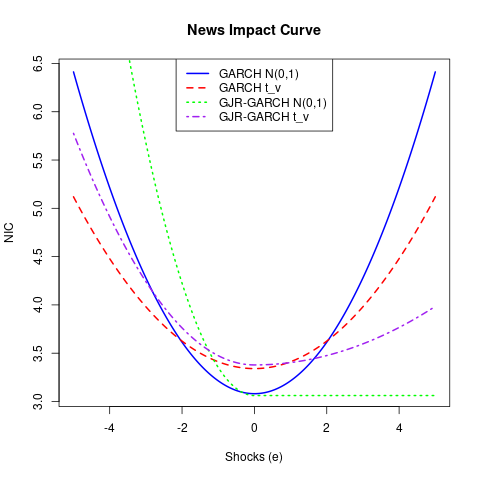
\includegraphics[width=0.35\textwidth]{../../docs/figures/NIC.png}
    \caption{News Impact Curve Plot}
    \label{fig:logreturn}
\end{figure}

\subsubsection*{Interpretation:}
Drawbacks of the GARCH models are obvious here, since the conditional variance is unable to respond asymmetrically to shocks in $y_{t}$, that is, a positive return has the same effect as a negative return upon variance. Since it is argued that negative innovations to shock returns tend to increase volatility more than positive innovations of the same magnitude. 

This plot offers a visual representation of the effect that new information has on the volatility predicted by different GARCH models. 
The standard GARCH model with normal innovations shows that the impact on conditional variance is symmetrical, both positive and negative shocks of the same magnitude have the same effect on predicted volatility, leaving the leverage effect unaccounted for. 

The GARCH model with a student's t-distribution is also symmetric but flatter compared to the standard GARCH model, indicating less sensitivity to shocks in general, due to the heavier tails in the t-distribution, reducing the impact of outliers. 

The GJR-GARCH model with normal distribution shows a pronounced asymmetry where negative shocks increase the conditional variance more than positive shocks. 
The model accounts for the leverage effect, where bad news influences volatility more than good news. 

The GJR-GARCH model with Student's t-distribution combines the properties of the GJR-GARCH with the heavier tails of the t-distribution. Showing an asymmetrical impact of shocks on volatility, similar to the GJR-GARCH but with the additional effect of heavier tails in the distribution of shocks. 
Heavier tails may imply that extreme values are more probable than in a normal distortion, and the impact curve is less steep for large magnitude shocks, indicating large shocks increase volatility less than what a normal distribution would suggest. 
Overall, both models with Student's t-distribution suggests that the models account for heavy tails in the distribution of shocks, whilst the GJR-GRACH models reveal an asymmetric response to shocks, highlighting the importance of the leverage effect. 

\subsection*{Question d}

\begin{table}[H]
\centering
\begin{tabular}{|l|c|c|}
\hline
\rowcolor{headercolor}
GARCH & Test statistic & P-value \\ 
\hline
Z & \zone & \pone \\ 
\hline
\(Z^2\) & \zfive & \pfive \\ 
\hline
\rowcolor{headercolor}
GARCH-t & Test statistic & P-value \\ 
\hline
Z & \ztwo & \ptwo \\ 
\hline
\(Z^2\) & \zsix & \psix \\ 
\hline
\end{tabular}
\quad % To add some spacing between the two tables
\begin{tabular}{|l|c|c|}
\hline
\rowcolor{headercolor}
GJR-GARCH & Test statistic & P-value \\ 
\hline
Z & \zthree & \pthree \\ 
\hline
\(Z^2\) &  \zseven & \pseven \\ 
\hline
\rowcolor{headercolor}
GJR-GARCH-t & Test statistic & P-value \\ 
\hline
Z & \zfour & \pfour \\ 
\hline
\(Z^2\) & \zeight & \peight \\ 
\hline
\end{tabular}
\end{table}

\subsubsection*{Interpretation:}

High p-values for the residuals indicate there is no statistical evidence to reject the null hypothesis that the residuals follow the respective distributions. 
Suggesting the residuals are white noise, meaning they are normally distributed with no autocorrelation. 

For the squared residuals, the p-values are high but slightly less so, again suggesting that there is no statistical evidence to reject the null hypothesis of no autocorrelation in the squared residuals. Indicating there is no ARCH effect and the conditional variance is well captured by the model. 

Whilst the LBQ p-values for the residuals are very high across all models, suggesting that none of the models leaves unexplained autocorrelation in the returns, which means that all models are adequate in this respect. 

The p-values for the squared residuals, which help to identify volatility clustering or ARCH effects, are also high across all models. 
However, in this context, the model with the highest p-value (corresponding to lowest test stat) for the square residuals is the GARCH-t model, indicating the least amount of autocorrelation and possibly the best fit among the compared models. 

\subsection*{Question e}

\begin{table}[H]
\centering
\begin{tabular}{|l|c|c|c|c|}
\hline
\rowcolor{gray!50}
& GARCH & GARCH-t & GJR-GARCH & GJR-GARCH-t \\
\hline
RMSFE & \rmsfei & \rmsfeii & \rmsfeiii & \rmsfeiv \\
\hline
DM Test statistic & NA & \dm & \dmi & \dmii \\
\hline
P-value & NA & \dmpii & \dmpiv & \dmpv \\
\hline
\end{tabular}
\end{table}

\subsubsection*{Interpretation:}

The RMSFE values indicate that GARCH+ has the smallest forecast error at 7.29, followed by GJR-GARCH-t at 7.30, GARCH at 7.32, and GJR-GARCH at 7.32. Lower RMSFE values suggest better forecast accuracy.

Diebold-Mariano (DM) Test results are only meaningful for GARCH+ and GJR-GARCH-t since GARCH is the benchmark. For GARCH+, the DM Test statistic is 2.00 with a p-value of 0.98, and for GJR-GARCH-t, the statistic is 1.83 with a p-value of 0.97. Since the p-values are much higher than the typical significance levels (e.g., 0.05 or 0.10), there's no statistical evidence that the forecast accuracy of GARCH+ and GJR-GARCH-t is different from GARCH.

Thus, although GARCH+ has a slightly lower RMSFE, the Diebold-Mariano test does not confirm its superiority over the benchmark GARCH model in terms of predictive accuracy. Economically, this suggests that there might be no practical benefit from using more complex models over the simpler GARCH model for forecasting this particular variance, as they do not provide statistically significant improvements in forecast accuracy.

\subsection*{Question f}
\subsubsection*{Interpretation:}

The choice of GARCH model involves a tradeoff between model misspecification and estimation noise. On one hand, simpler models like the standard GARCH have fewer parameters and are less prone to estimation noise, but may suffer from misspecification if the true volatility process exhibits features that the model cannot capture (e.g., asymmetry, time-varying volatility).

More flexible models like the GJR-GARCH or GARCH with additional components (GARCH+) can potentially better fit the data by accounting for these complexities, reducing misspecification. However, they require estimating more parameters, introducing greater estimation noise.

While complex models offer an improved in-sample fit, they do not necessarily outperform simpler models in out-of-sample forecasting due to the increased estimation noise. The benefits of reduced misspecification may be offset by the noise from estimating additional parameters, especially in small samples.

Ultimately, the optimal model balances the competing goals of parsimony and flexibility. Simple models are preferred when estimation noise is a greater concern, while more complex specifications are justified if the true data-generating process exhibits features that warrant additional modeling components, even at the cost of some estimation noise.

Model selection criteria like information criteria aim to navigate this tradeoff by penalizing overly complex models. However, the final choice depends on the relative importance of in-sample fit versus out-of-sample forecasting performance for the specific application.

\newpage
\section*{Appendix}

For reproduction of said script, see \url{https://github.com/oddish3/FE-CW/tree/master}

\lstinputlisting[language=R]{../../code/Script.R}




\end{document}

